ection{Experimental Evaluation}
\subsection{Datasets and evaluation protocol} \label{eval:protocol}
Our default dataset in this paper will be INRIA \emph{Holidays} dataset \cite{holidays}. This dataset consists of 1491 images divided in 500 groups of matching images. For the remaining of this report, if the dataset of an experiment is not mentioned, the experiment is performed on \emph{Holidays}.
We also perform in the \emph{Oxford} dataset \cite{oxford}, which consists of 5062 images separated in 55 groups of matching images.

Each group of these datasets contains one query image. 
For each query image, we calculate its similarity to all other images in the database and rank them, in decreasing order. 
The average precision of a group is calculated by the ranking of the images of the group for the similarity with the corresponding query image. 
The final mean average precision (mAP) for a dataset is the mean of the average precision over all its groups.
As negative sample of images, we use a set of images $10^5$ from Flickr \cite{oxford}. 
For a full rank decomposition, we use a subset of Flickr100k, between $6000$ and 15000 images. 
As stated in section \ref{low-rank} and further discussed in section \ref{time-scale}, a full rank decomposition does not scale well for bigger number of negative samples. For low rank decomposition, we use all 100000 images.

At evaluation time, for a dataset that consists of $p$ images and $q$ query images, we calculate its $p\times q$ \emph{similarity matrix} $S$, where each of its $q$ columns is the matching scores of the query image with all the $p$ images.


\subsection{Which kernel to choose?}
We tested four different kernels: linear kernel, RBF kernel, polynomial kernel and spatial pyramid match kernel. Each kernel takes as parameter a scalar $\gamma$.

\begin{align}
    &k_{linear}(x,y) = x^Ty; \label{k:lin}\\
    &k_{rbf}(x,y) = \exp(-\gamma|\! |x-y|\! |^2); \label{k:rbf}\\
    &k_{poly}(x,y) = x^Ty+\gamma(x^Ty)^2; \label{k:poly}\\
    &k_{spp}(x,y) = \dfrac{1}{2^L}\mathcal{I}(H^0_x, H^0_y) +\sum_{l=1}^L\dfrac{1}{2^{L-l+1}}\mathcal{I}(H^{l,_gamma}_x, H^{l,\gamma}_y). \label{k:spm}
\end{align}
\textbf{Linear SLEM} The linear kernel of Equation (\ref{k:lin}) is the first default choice and equivalent to the non-kernelized version of SLEM.
In the remaining of this paper, we reference to linear SLEM when we use the non-kernelized SLEM.
\textbf{Gaussian SLEM} The radial basis function kernel of Equation (\ref{k:rbf}) is a
well known reproducing kernel, used for classification with support vector machines.
\textbf{Polynomial SLEM} The polynomial kernel of Equation (\ref{k:poly}) is a reproducing kernel normally used in natural language processing. 
This three kernels are amount the most used kernels in the machine learning literature.
\textbf{SPM SLEM} The pyramid match kernel of Equation (\ref{k:spm}) is a Mercer kernel introduced in \ref{GrauDa05} 



\subsection{Base visual features}
Local descriptors: RootSIFT \cite{3things} and deep convolutional features \cite{SimonZisser15}

Embedding: VLAD features \cite{VLAD} and aggregation \cite{babenko15}

Caffe CNN features \cite{jia2014caffe}


%We use four base features as the representation in $\RR^d$ of our images. Firstly, we use VLAD features, as used in \cite{ZePe15}. 
%CNN features are non-negative and can be used both as $\mathbb{L}^1$ or $\mathbb{L}^2$ normalized features. The third features are spatial pyramids of SIFT descriptors, as used in \cite{spk}. These are non-negative $\mathbb{L}^1$ normalized features. \emph{\color{red} Details of these features construction are not relevant right now.}


\subsection{Implementation details}
\emph{\color{red} Not relevant right now.  To be written.}
$8192$ dimensional VLAD features.

E-SVM: $0.6$ second to solve one single exemplar.

SLEM: $30$ seconds to solve a $8192\times 8192$ linear system for all exemplars of the dataset.

Kernelized SLEM: at most $0.3$ seconds (for RBF kernel) for each iteration of (\ref{icd:algo}) algorithm plus at most $30$ seconds to solve a $r'\times r'$ system.


\subsection{Full rank results}

\begin{table*}[t]
\begin{center}
\begin{tabular}{|c|c|c|c|c|c|}
\hline
Method, features & VLAD-64 \cite{VLAD}& CNN \cite{jia2014caffe} & Root-SIFT \cite{3things} & SPoC CNN \cite{babenko15} &  SP-CNN \cite{SPPCNN} \\
\hline\hline
Baseline            & 72.7 & 68.2 & 37.4 & 73.1 & 64.7\\
%Whitening           & -    & -    & -    & -    & -\\
LDA                 & 69.4 & 69.2 & -    & 77.5 & -\\
E-SVM               & 77.5 & 71.3 & 40.1 & 79.8 & 64.7 \\
Linear SLEM         & 78   & 72.1 & 38.2 & 78.3 & 68 \\
Gaussian SLEM       & 78.1 & 72.9 & 39.7 & 81.4 & 68.6 \\
Poly SLEM           & 78.1 & 72.9 & -    & 82   &   -   \\
SPM SLEM            & -    & 70.2 & 66.9 & -    & 70.2 \\
\hline
\end{tabular}
\end{center}
\caption{Mean average precision results for INRIA Holidays dataset, expressed as percentages. The - means the tests can not be performed or was not performed yet.}
\end{table*}


\begin{table*}[t]
\begin{center}
\begin{tabular}{|c|c|c|c|c|c|}
\hline
Method, features & VLAD-64 \cite{VLAD}& CNN \cite{jia2014caffe} & SP-SIFT \cite{spk} & SPoC CNN \cite{babenko15} &  SP-CNN \cite{SPPCNN} \\
\hline\hline
Baseline            & 46.3 & 40.6 & - & 54.4 & 44 \\
%Whitening           & 07   & 20.2 & - & -    & -\\
LDA                 & 50.9 & 45   & - & 63.7 & 37.4\\
E-SVM               & 57.5 & 44.6 & - & 62.1 & - \\
Linear SLEM         & 57.5 & 45.5 & - & 64.1 & 45 \\
Gaussian SLEM       & 59   & 46.1 & - & 64.9 & 45 (no cv) \\
Intersection SLEM   & -    & 42.2 & - & -    & - \\
\hline
\end{tabular}
\end{center}
\caption{Mean average precision results for Oxford 5k buildings dataset, expressed as percentages. The - means the tests can not be performed or was not performed yet.}
\end{table*}


\subsection{Time Scalability} \label{time-scale}
\begin{figure}[!h]
\centering
\begin{subfigure}[b]{0.32\textwidth}
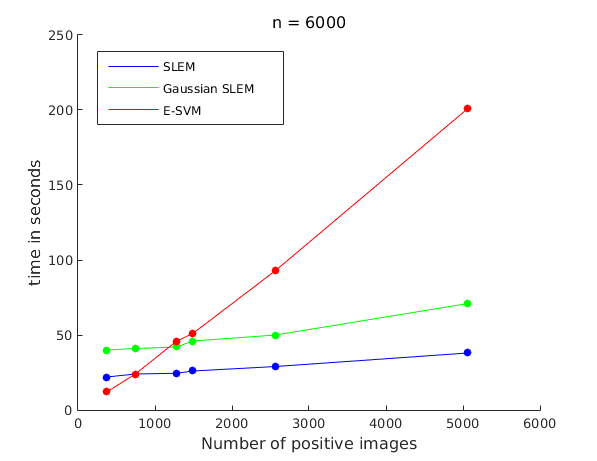
\includegraphics[width=\textwidth]{speed_n_6K.png}
\end{subfigure}
\begin{subfigure}[b]{0.32\textwidth}
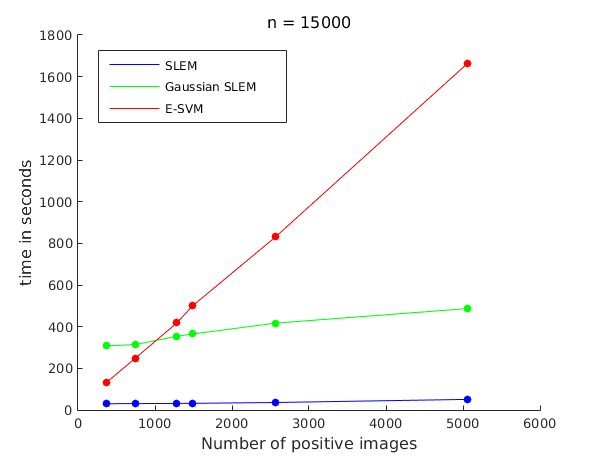
\includegraphics[width=\textwidth]{speed_n_15K.png}
\end{subfigure}
\begin{subfigure}[b]{0.32\textwidth}
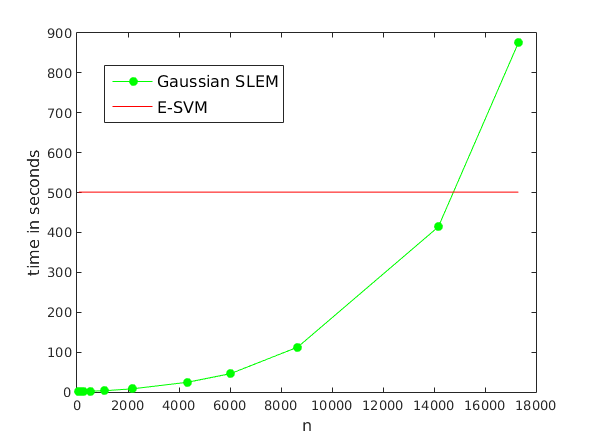
\includegraphics[width=\textwidth]{speed_n.png}
\end{subfigure}
\caption{Comparison between time calculation feature encoding for different methods. At left, we use $n=6000$ negative examples. At right, $n=15000$ negative examples. In both experiments, we use VLAD as base features.}
\label{time:scalar}
\end{figure}

\subsection{Low-rank decomposition evaluation}

\begin{figure}[!h]
\centering
\begin{subfigure}[b]{0.48\textwidth}
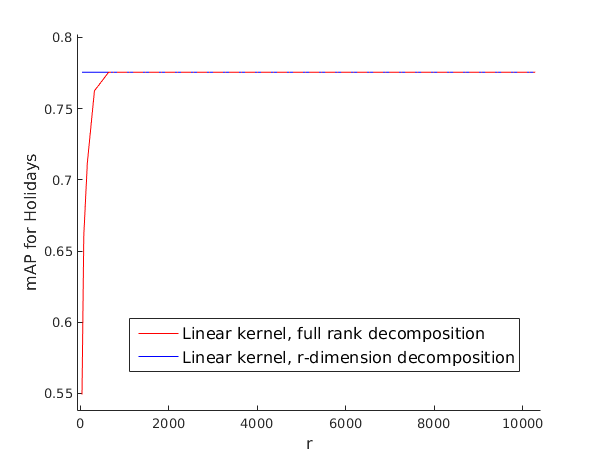
\includegraphics[width=\textwidth]{linear_decomposition_nolog.png}
\end{subfigure}
\begin{subfigure}[b]{0.48\textwidth}
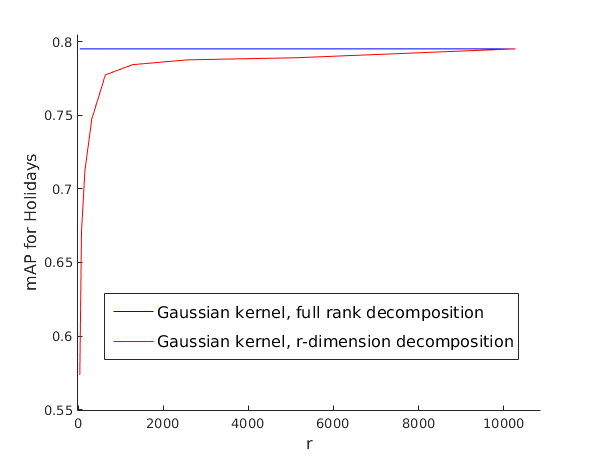
\includegraphics[width=\textwidth]{rbf_decomposition_nolog.png}
\end{subfigure}
\caption{Comparison between full rank and low rank. In blue, mAP results for 

At the left, comparison between no kernel results and linear kernel results. In black, mAP of non kernelized SLEM. In red, mAP for different low-rank decompositions of linear kernel matrix. In this experiment, $r=2^{13}$ and we set $\log_2 r'$ in $\{6, 7,...,13\}$. At the right, comparision between the gaussian kernel results and its low-rank decomposition results. In blue, mAP of the full-rank Gaussian SLEM. In red, mAP for different low-rank decomposition of Gaussian SLEM. In this experiment, $r=10281$.}
\label{no.ker.vs.linear2}
\end{figure}

%\caption{Comparison between no kernel results and linear kernel results. In black, mAP of non kernelized SLEM. In red, mAP for different low-rank decompositions of linear kernel matrix. In this experiment, $r=2^{13}$ and we set $\log_2 r'$ in $\{6, 7,...,13\}$. }

%\caption{Comparison between no kernel results and linear kernel results. In black, mAP of non kernelized SLEM. In red, mAP for different low-rank decompositions of linear kernel matrix. In this experiment, $r=2^{13}$ and we set $\log_2 r'$ in $\{6, 7,...,13\}$. }


